\chapter[SCP-023 黑煞星]{
    SCP-023 Black Shuck\\
    SCP-023 黑煞星
}

\label{chap:SCP-023}

\begin{figure}[H]
    \centering
    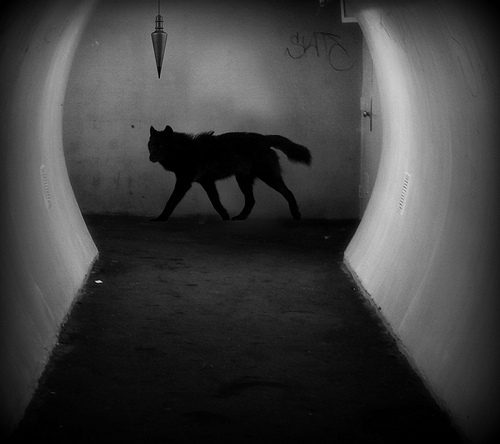
\includegraphics[width=0.5\linewidth]{images/SCP.023.jpg}
    \caption*{SCP-023於SCP-███逃脫事件中收容於暫時收容區}
\end{figure}

\bb{項目編號:}SCP-023

\bb{項目等級:}Euclid

\bb{特殊收容措施:}\dd{SCP-023應收容於一間5X5米的標準收容單位內。} SCP-023收容於Site-██的一處收容區,該區結構為兩道迴廊交錯構成的叉狀建物,並延邊緣圍起圍牆; 四端任一走道的長度皆長於3米,且參號及肆號迴廊端點除了正常的門外,也附加了假門。監視攝影機設於四端端點的門上方。

不論何時,SCP-023的兩個眼窩應以硬橡膠制的球狀眼部植入物填充。當植入物有劣化的情形時,必須進行更換。劣化情形可依在監視平台觀察到的"火光"亮度來判別。當亮度超過██燭光時,必須於12小時內更換植入物。更換時應注意,只能在完全日落後進行更換,且不可同時更換兩側的植入物。任何人員不可在任何時間直視SCP-023的眼窩內部。

依據\hyperref[sec:DOC-incident-023-27]{事件報告023-27},所有具有反光面的物品,如顯示器,螢幕,或任何一種眼鏡,皆不允許出現在SCP-023的收容區半徑30米內。上述要求亦包括連線至監視攝影機的螢幕零部件。於收容區外定點哨點的保安人員亦強制遵行上述要求。

關於SCP-023的相關試驗皆已無限期推延。

\bb{描述:}SCP-023是一隻大型無性別的黑色長毛犬科生物(肩高1.5米),\dd{有一對亮橘紅色的\mbox{\hyperref[chap:TAIL-mothers-love]{眼睛}}跟一口突出的牙齒}(見\hyperref[sec:DOC-incident-report-023-26]{事件報告023-26})。 當一位個體與SCP-023發生視線接觸時,自視線錯開起約1年內,該個體或個體的近親親屬之一將會死亡。盡管更進一步的試驗皆已無限期推延,但依據當前資料,個體死亡的機率會比個體的親屬高,且受害者之間沒有明顯的特殊相關性,也沒有發現有特別偏向某類受害者的情形。這可能表示SCP-023的受害者是完全隨機的, 然而無法得知之前試驗資料的受害者是死於1年期間的初期或是末期。試圖在1年末期前,處決所有有過與SCP-023視線接觸的個體及其親屬們的行動,因[資料刪除]而結束。

SCP-023的受害者經驗屍後發現,他們的外觀毫無受傷痕跡,然而其餘部份已被經高度壓縮過的灰燼“填滿”;其餘部份包括但不限於任何器官組織及循環系統。所有受害人的肌肉組織,骨骼及腦組織皆有暴露於攝氏██度以上的跡象。

SCP-023如被收容於外觀不是近似於“十字路口”的設施時,牠將能傳躍出牆外,到達最近距離且符合收容條件的地區,並焚化路徑上所有物質。

基金會首次注意到SCP-023是在███████的一座教堂,當時牠在集會中發起一次攻擊,直接殺害 █位平民,並因視線接觸而[已刪節]。於回收SCP-023後,所有證人及倖存者皆施以B級記憶清除。該次事故已掩飾為縱火案件。

\bb{附錄023-001}\\
在██\slash ██\slash ████,SCP-023穿牆脫出收容區(事故報告023-01)。之後於Site-███內兩道迴廊的交叉口發現。特工█████ 注意到SCP-023看起來很像[已刪節]。SCP-023的特殊收容措施已更新。研究助理███████因此次過失受到申誡。

\bb{附錄023-002}\\
自10\slash 12\slash ██94第一次收容以來,已有 ███ 位工作人員及██位平民的死亡歸因於SCP-023。

\bb{附錄023-003:}\\
正在評估升至Keter的請求。

\bb{附錄023-004:}\\\hyperref[chap:SCP-1111]{SCP-1111-1}和SCP-023可能是同一现象的两个变体,因为它们被发现具有几个相同的特性:对地理位置的敏感性、具有破坏性、类似的犬类外观。对这一现象的深入调查正在进行中。由于SCP-1111-1无法捕获,研究目前集中在SCP-023上。

\chapter{
    事件报告 023-27
}

\label{chap:DOC-incident-023-27}

\bb{涉及SCP:}\hyperref[chap:SCP-023]{SCP-023}

\bb{涉及人员:}████博士,[数据删除]

\bb{日期:}██\slash ██\slash ██

\bb{地点:}Site-██

\bb{描述:}时间线:

00:00:10 – 两(2)个D级人员把一对玻璃眼球装进SCP-023的眼眶。

00:00:15 – 玻璃眼珠呈现出一种橘红色,与SCP-023被摘除的眼睛看起来一样。

00:03:13 – SCP-023的眼窝流出了熔化的玻璃。

00:05:54 – [数据删除]出现在了Site-██所有的镜头,窗户,镜子,监视器,以及玻璃表面。

00:06:12 – Site-██紧急疏散。

06:54:07 – 日出。派出D级人员检查SCP-023的周围局域。 [数据删除]消失了。SCP-023仅留下了一滩熔化的彩色玻璃及其周围烧焦的地板。

\hr

\bb{个人日志:}████博士

\bb{日期: ██\slash ██\slash ████}

都是我的错。我造成了我的研究团队和机构的失败。唯一能做的只有继续尝试了。我们必须收容SCP-023。

\bb{备注:} 在 ██\slash ██\slash ████,事件023-27发生的一年后,███人员被葬在了Site-██ 外围的大型墓地中。


\section{事件报告 023-26}

\label{sec:DOC-incident-report-023-26}

\bb{涉及SCP:}\hyperref[chap:SCP-023]{SCP-023}

\bb{涉及人员:}████████博士,五(5)位D级人员

\bb{日期:}██\slash ██\slash ██ - ██\slash ██\slash ██

\bb{地点:}Site██

\bb{描述:}

为了减少SCP-023带来的危险,████████博士已获准去除023的眼睛和牙齿。在它的眼睛被移除后,SCP-023完全消失,突破了收容。下午4:37,SCP-023在一段洲际公路上被重新发现并被带回了收容区,由D级人员继续完成拔牙的工作。这段时间内暴露在SCP-023面前的平民人数未知,死亡记录仪监测到了九(9)位平民的死亡或与此次事件有关。

对SCP-023接下来48小时的实时监测证明了它只在Site██外可见到太阳时才会消失。

\bb{附录-023-026-1:}

在██\slash ██\slash ████,████████博士因对于事件023-026的直接或间接责任已受到停职审查的处分。████博士现在负责SCP-023。

\ii{此次事件增加了收容的难度,因此████████博士的遭遇应该提醒基金会的所有成员,基金会的目标是:控制,收容,保护。而研究、实验、便利性,甚至基金会成员的个人安全都是次要的。我们的工作不是保护自己。}

O5-██

\bb{附录-023-026-2:}事件023-26发生的一年后,总计█具尸体被认定与SCP-023的暴露有关。

